\chapter{Introduction}

\begin{flushleft}
The circle is arguably the most fundamentally studied mathematical object in history. In fact, the construction of the unit circle dates all the way back to the second century BC \cite{unit_circle}. With this elementary object, we are able obtain two trigonometric functions, enabling us to study a myriad of physical processes such as the motion of waves and the oscillatory properties of pendulums. In this project however, we will be looking less at the properties of the circle, and more on various geometries involved when we attempt to group, or \textit{pack} as many as we can together. 
\end{flushleft}

\begin{flushleft}
As some motivation for what is to come, let's take a stroll down the fruits and vegetables section at the supermarket. While looking around, we notice that spherical fruit, such as oranges, are stacked high in a in a pyramidal-like shape that tapers off at the top. A display like this is known as a \textit{face-centered cubic packing}.
\end{flushleft}

\begin{figure}[htbp]
    \centering
    \begin{tabular}{c c}
      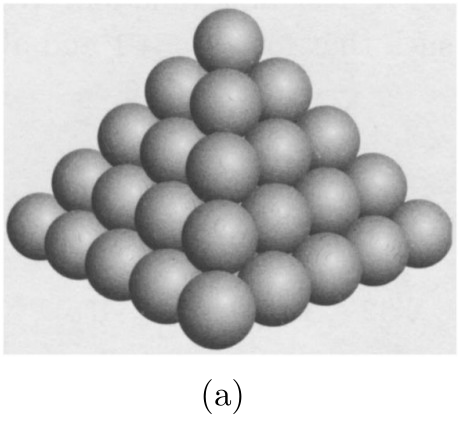
\includegraphics[width = 0.35\textwidth]{Chapter 1/2. Cubic packing.png}   & 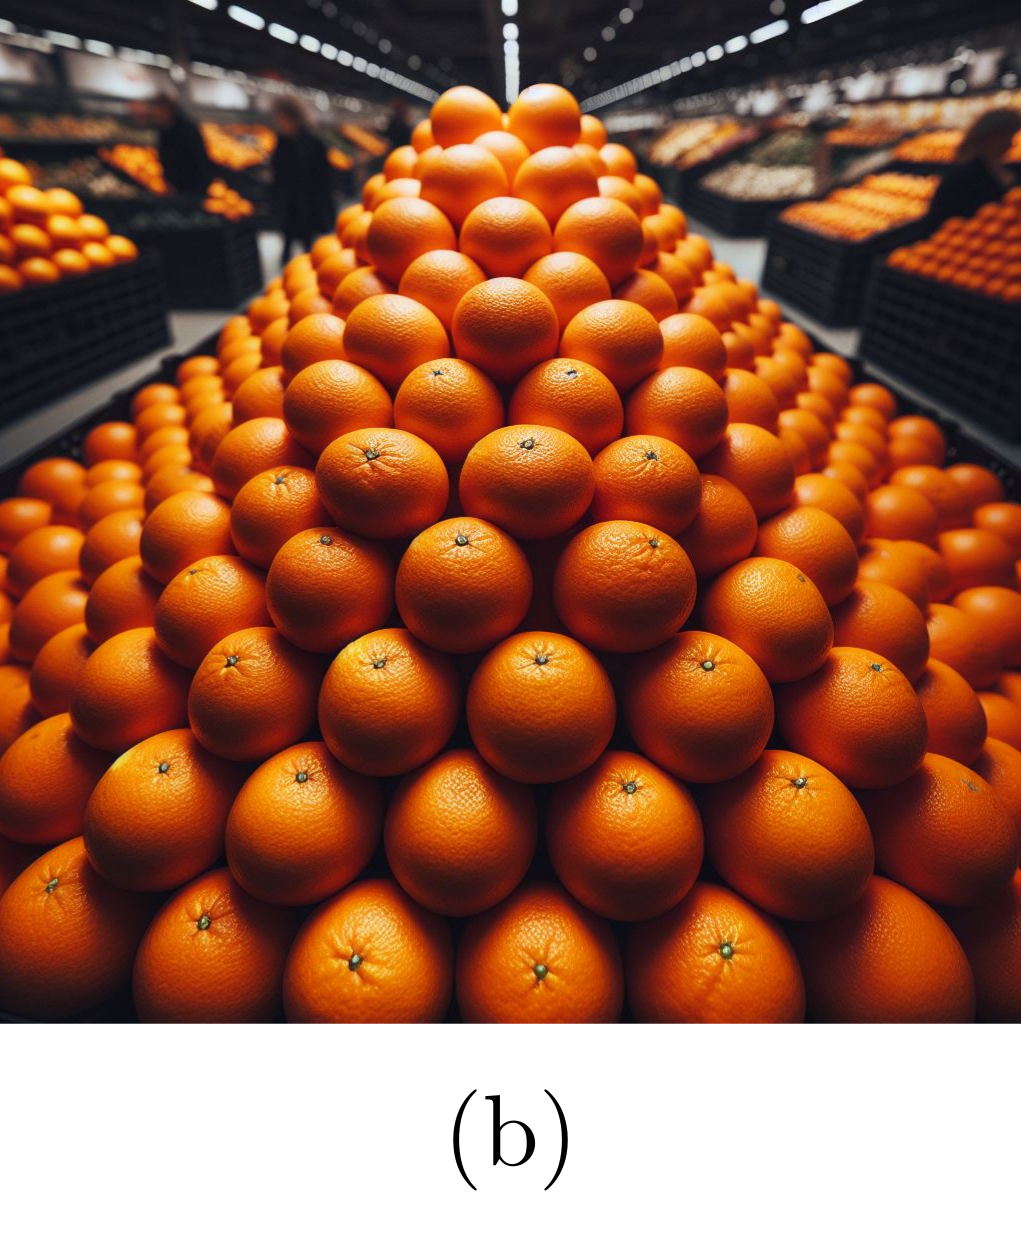
\includegraphics[width = 0.275\textwidth]{Chapter 1/oranges.png}
    \end{tabular}
    \caption{(a) A face-centered cubic packing, taken from \cite{kepler}. (b) An image of oranges stacked in a face-centered cubic packing, generated by DALL·E 3.}
\end{figure}
\vspace{-4 mm}
\begin{flushleft}
This interesting observation was studied by Johannes Kepler, who attempted to find the optimal way to stack cannonballs. In 1611, Kepler conjectured that a face-centered cubic packing is the most efficient method to stack spheres in 3-dimensional space. This was proved by Thomas Hales, at first using computational methods in 1998, and a formal proof was accepted in 2017 \cite{Kepler_proof}.
\end{flushleft}

\begin{flushleft}
Going back to the 2-dimensional circle, our interest lies in a \textit{circle packing}, which involves arranging several circles in the plane such that they may only touch tangentially, and there is no overlap between any of the circles. By imposing different constraints, we can generate circle packings where the arrangement formed has circles packed together with a variety of radii, producing an aesthetically pleasing image to regard. They can also be used to study the world around us under a different lens. An example of this involves modelling the arrangement of particles in a crystalline structure as a tight packing of circles \cite{crystalline}.
\end{flushleft}

\begin{flushleft}
We can study circle packings using similar computational methods, as this project will illustrate. By marking the center of each circle, and joining centers with a line if the circles they inhabit are tangential to each other, we are able to construct the packing's \textit{contact graph}, effectively converting our geometric problem into a graph theoretic one. This allows us to use tools from Graph Theory, increasing the size of our repertoire.    
\end{flushleft}

\begin{figure}[htbp]
    \centering
    \begin{tabular}{c c}
        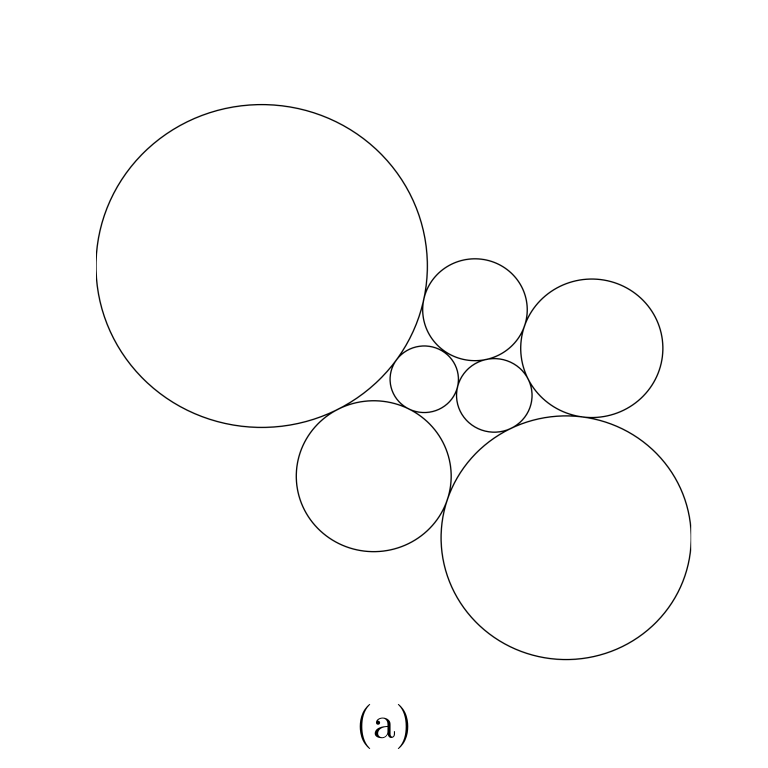
\includegraphics[width = 0.4\textwidth]{Chapter 1/packing.png} & 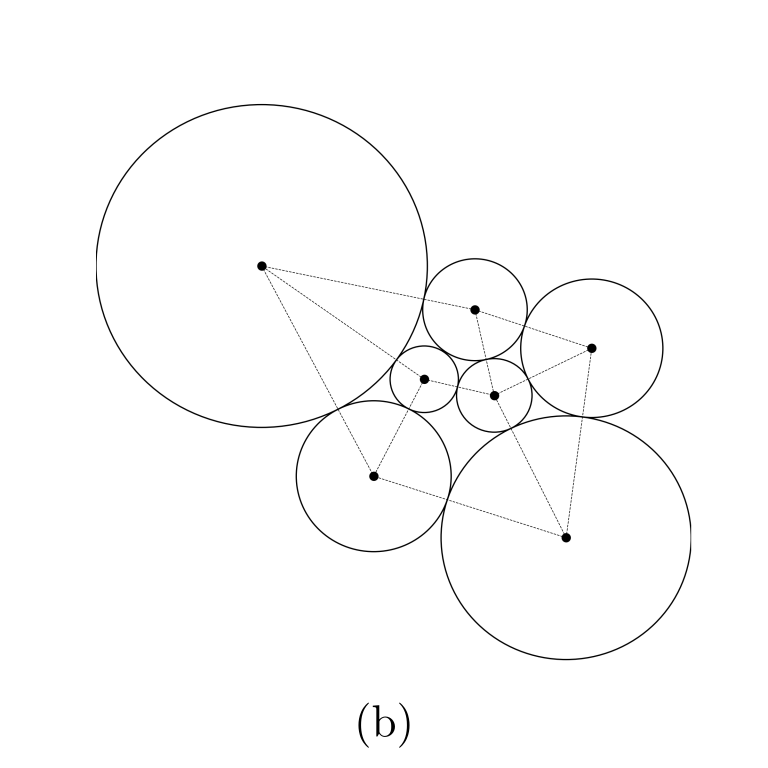
\includegraphics[width = 0.4\textwidth]{Chapter 1/packing_contact.png}   
    \end{tabular}
    \caption{(a) A circle packing with 7 circles. (b) The packing with its contact graph visualized.}
\end{figure}
\vspace{-2 mm}
\begin{flushleft}
One such property, and the main focus of this project, is \textit{rigidity}, which was first studied by James Clerk Maxwell. Rigidity is a measure of how `stiff' something is. Consider structures such as buildings, bridges, sandcastles and so on. Some of them hold up, whereas others don't. This is partly due to the material it is made from, and also because of the fact that some of these structures are rigid, while others are not.     
\end{flushleft}

\begin{flushleft}
In this project, we will be introduced to the ideas of rigidity, what it means for a \textit{framework} to be rigid, and how we can study the rigidity of circle packings. Along the way, we will try to gain some insight to the question that this thesis focuses on:

\begin{center}
    \textit{``For every planar and minimally rigid graph, does there exist a circle packing that is also infinitesimally rigid?''}
\end{center}
\end{flushleft}

\begin{flushleft}
An exciting aspect of this project is the way in which various fields within mathematics become involved when studying something that seems purely geometric. Ideas from Graph Theory and Linear Algebra come into play and therefore, the intended audience for this project are mathematics students that are accustomed to some fundamental ideas from these two fields, as well as a basic understanding of how to code. That being said however, everything will be clearly defined and explained as we come across it. Moreover, all the code involved in this project can be viewed on Github at \href{https://github.com/Titwik/Dissertation}{Titwik/Dissertation}.    
\end{flushleft}

\begin{flushleft}
The only pre-requisite required to understand the content of this project involves some fundamental linear algebra. Specifically, the knowledge of how vectors work, and a good understanding of matrices and their properties. The interested reader can explore the flavor of mathematics involved in this project in texts relating to;
\begin{itemize}
    \item \textit{Graph Theory}: The study of mathematical structures, known as graphs, that represent relationships between objects. It has several applications, some of which include computer science, biology and logistics to name a few.
    \item \textit{Discrete Mathematics}: The study of countable, discrete objects rather than continuous quantities. Topics involved include Set Theory and Logic, and it plays a big role in the study of computer science.
    \item \textit{Constrained Optimization}: Attempting to find the maximum or minimum of a certain `objective' function while adhering to specific constraints. 
\end{itemize}
\end{flushleft}

\begin{flushleft}
With all that said, let's get into it!    
\end{flushleft}

